
\documentclass[preprint,12pt]{elsarticle}
\makeatletter
\def\ps@pprintTitle{%
 \let\@oddhead\@empty
 \let\@evenhead\@empty
 \def\@oddfoot{\centerline{\thepage}}%
 \let\@evenfoot\@oddfoot}
\makeatother
\usepackage[spanish]{babel}
\usepackage{amssymb}
\usepackage{graphicx}
\usepackage{lineno}
\usepackage[utf8]{inputenc}
\usepackage{url}
\usepackage{natbib} 
\usepackage{amsmath} 
\usepackage{amssymb} 

\begin{document}
	\begin{frontmatter}
		\title{\huge Informe de Laboratorio Nro 08 : Instalación de un Gestor de Base de Datos Oracle}
		\address{Universidad Privada de Tacna}
		\address{Escuela Profesional de Ingeniería de Sistemas}
		\address{Curso : Base de Datos II}		
		\author{Jose Luis Quispe Mamani             	(2015053235)}		
		\address{Tacna, Perú}
\end{frontmatter}

%% INFORMACIÓN GENERAL -----------------------------------------------------------------------------------------------------------------------------------
\section{INFORMACIÓN GENERAL}
Objetivos:
\begin{itemize}
\item Crear un contenedor de la imagen de Oracle Database Enterprise Edition 
\item Desplegar una base de datos usando un contenedor Oracle Database
\end{itemize}
Equipos y programas utilizados:
Para el siguiente laboratorio requerimos de:
\begin{itemize}
\item Computadora con sistema operativo Windows 10
\item Docker Desktop
\item Oracle SQL Developer for Windows

\end{itemize}

%% MARCO TEORICO -----------------------------------------------------------------------------------------------------------------------------------
\section{MARCO TEÓRICO}
\begin{itemize}
\item Las herramientas del contenedor, como Docker, ofrecen un modelo de implementación basado en imágenes. Esto permite compartir una aplicación, o un conjunto de servicios, con todas sus dependencias en varios entornos.
\item Docker: Es un proyecto de código abierto que automatiza el despliegue de aplicaciones dentro de contenedores de software, proporcionando una capa adicional de abstracción y automatización de virtualización de aplicaciones en múltiples sistemas operativos.
\end{itemize}

%% PROCEDIMIENTO -----------------------------------------------------------------------------------------------------------------------------------
\section{PROCEDIMIENTO}
\textbf{Paso 1 : Iniciando Docker}
\begin{enumerate}[a)]
\item Hacemos doble clic en el acceso directo "Docker Desktop" para inciar Docker. Luego presionamos clic derecho sobre el icono y seleccionamos la opción "Sig In".
\begin{figure}[htb]
	
\end{figure}
\item Ingresamos nuestras credenciales usuario  y contraseña.

\textbf{Paso 2 : Creando un contenedor con Oracle Database para Linux}
\item En un navegador de internet accedemos a la dirección "https://hub.docker.com/" .\newline 
Iniciamos sesión.
\begin{figure}[htb]
	
\end{figure}

\item Buscamos el repositorio para Oracle Database Enterprise Edition.
\begin{figure}[htb]

\end{figure}

\item Procedemos a seleccionar la opción "Proceed to Checkout" e ingresamos los datos solicitados por el formulario y aceptamos lo términos de acuerdo.
\begin{figure}[htb]
	
\end{figure}

\item En la ventana nueva copiamos el comando que se encuentra dentro del reacuadro plomo.
\begin{center}docker pull store/oracle/database-enterprise...\end{center}
\begin{figure}[htb]
	\begin{center}
		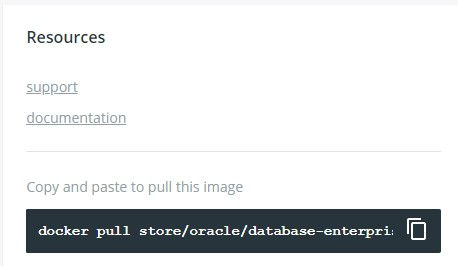
\includegraphics[width=8cm]{./IMAGENES/Docker8_04}
	\end{center}
\end{figure}
\item En la venta de PowerShell, escribir el siguiente comando:
\begin{center}docker login\end{center}
\begin{figure}[htb]
	\begin{center}
		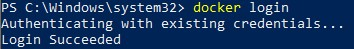
\includegraphics[width=8cm]{./IMAGENES/Docker8_20}
	\end{center}
\end{figure}
\item Copiamos el comando en la aplicación PowerShell. \begin{center}docker pull store/oracle/database-enterprise:12.2.0.1\end{center}
El comando descargará la imagen del contenedor de Oracle Database en un servidor Linux y mostrará la siguiente resultado.
\begin{figure}[htb]
	\begin{center}
		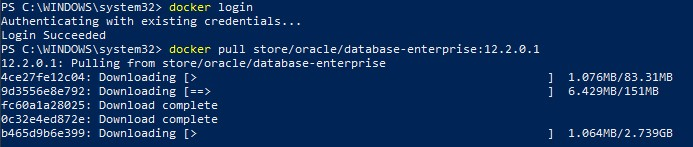
\includegraphics[width=12cm]{./IMAGENES/Docker8_06}
		\caption{Descargando la imagen de Oracle Database}
		\bigskip
		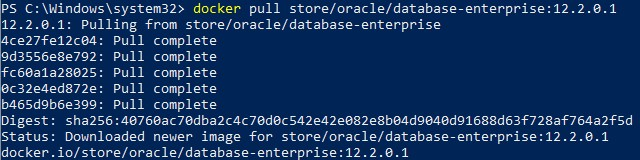
\includegraphics[width=12cm]{./IMAGENES/Docker8_07}
	\end{center}
\end{figure}


\item Seguidamente ejecutar el comando :\newline
docker run -d -it --name ORACLEDB01 -p 1521:1521 -p 5500:5500 store/oracle/database-enterprise:12.2.0.1
\begin{figure}[htb]
	\begin{center}
		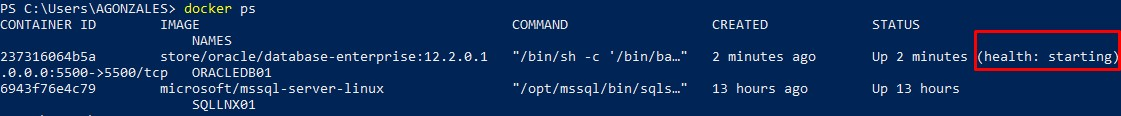
\includegraphics[width=12cm]{./IMAGENES/Docker8_11}
	\end{center}
\end{figure}
\item Ejecutamos el comando docker ps . Y nos devolverá el ID del contenedor.
\begin{center}
237316064b5a54649571720eafa8aeab3c0f14c9ee86b5386a97832ff201faf0
\end{center}

\item Cuando el estado del contenedor sea "healthy", en la consola de PowerShell, ejecutamos el siguiente comando:
\begin{center} docker exec -it ORACLEDB01 bash -c "source /home/oracle/.bashrc;sqlplus / as sysdba \end{center}
\begin{figure}[htb]
	\begin{center}
		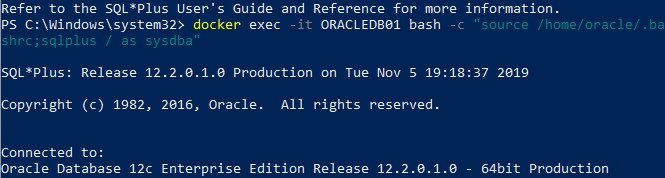
\includegraphics[width=12cm]{./IMAGENES/Docker8_08}
	\end{center}
\end{figure}

\item En la línea de comentados de SQLPLUS , escribir lo siguiente:
\begin{figure}[htb]
	\begin{center}
		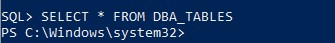
\includegraphics[width=7cm]{./IMAGENES/Docker8_12}
	\end{center}
\end{figure}
Visualizará una serie de registros que representan las tablas del rol DBA\newline
Escribir el comando quit para cerrar la sesión de SQLPLUS

\item En una pestaña nueva del navegador de internet acceder a la siguiente dirección https://localhosts:5500/em. Seleccionar la opción Acceder al localhost (sitio no seguro).
\begin{figure}[htb]
	\begin{center}
		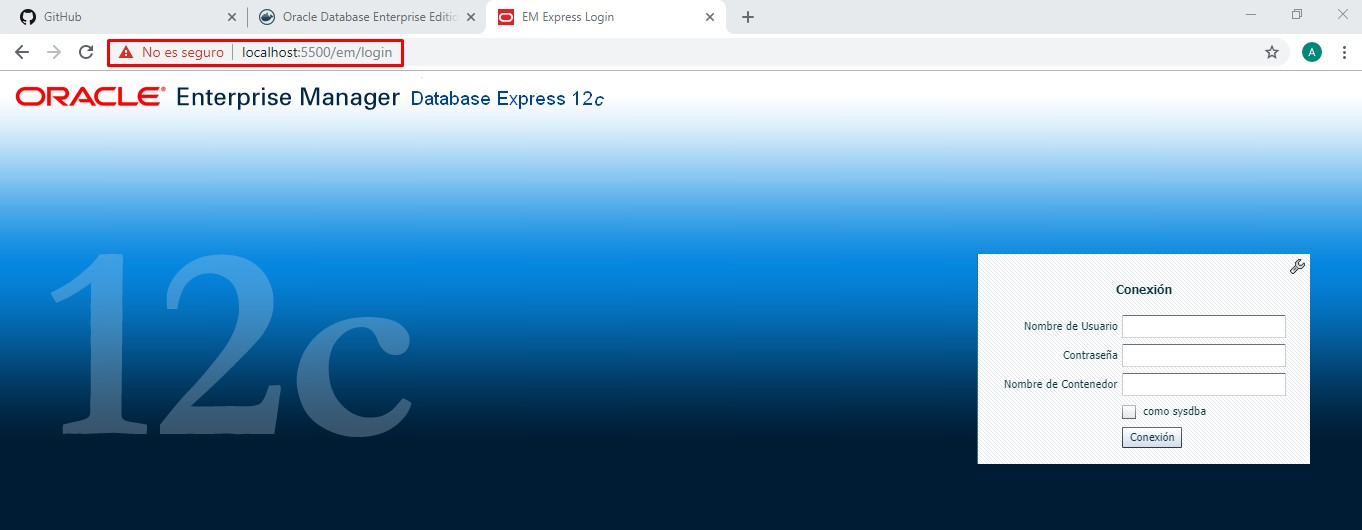
\includegraphics[width=12cm]{./IMAGENES/Docker8_13}
	\end{center}
\end{figure}

\item Iniciar sesión con los siguientes datos:
\begin{center}Usuario:sys\end{center}
\begin{center}Contraseña: Oradocdb1\end{center}
\begin{center}Marcar check como sysdba\end{center}
\begin{figure}[htb]
	\begin{center}
		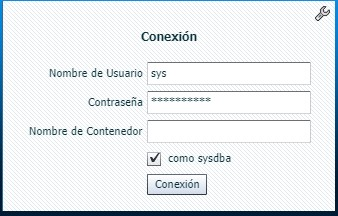
\includegraphics[width=6cm]{./IMAGENES/Docker8_14}
	\end{center}
\end{figure}

Luego se visualizará la siguiente ventana
\begin{figure}[htb]
	\begin{center}
		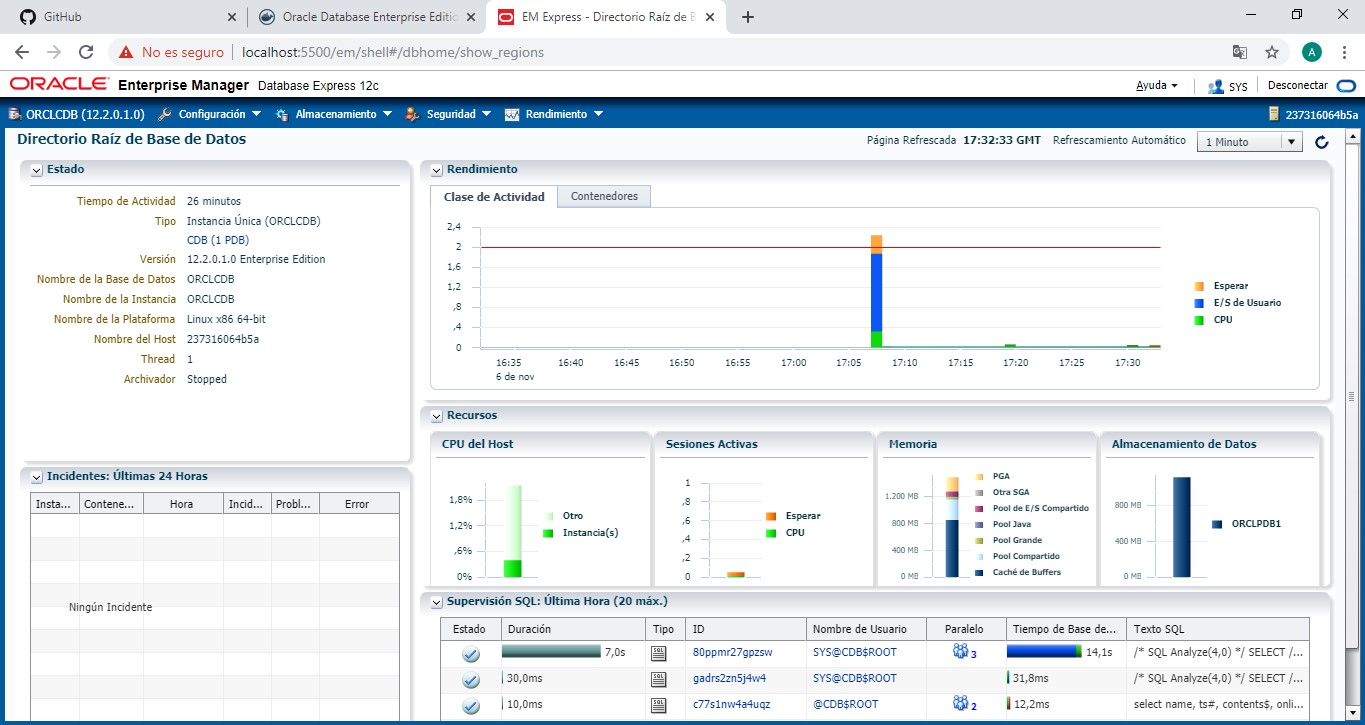
\includegraphics[width=13cm]{./IMAGENES/Docker8_16}
	\end{center}
\end{figure}


\textbf{Paso 3 : Adicionando persistencia}
\item En PowerShell ejecutar el siguiente comando\newline
\begin{figure}[htb]
	\begin{center}
		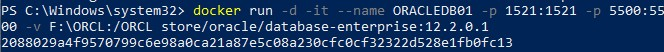
\includegraphics[width=13cm]{./IMAGENES/Docker8_17}
	\end{center}
\end{figure}
\item En el directorio especificado F:/ORCL se creará las siguientes carpetas.Correspondientes al contenerdor Oracle Database.
\begin{figure}[htb]
	\begin{center}
		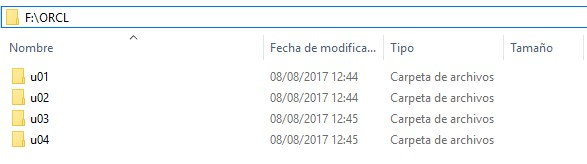
\includegraphics[width=13cm]{./IMAGENES/Docker8_18}
	\end{center}
\end{figure}
\end{enumerate}

%% ANÁLISIS E INTERPRETACIÓN DE RESULTADOS -----------------------------------------------------------------------------------------------------------------------------------
\section{ANÁLISIS E INTERPRETACIÓN DE RESULTADOS}
\begin{enumerate}[a)]
\item Con el comando para iniciar con un contenedor podemos asignar los siguientes parámetros:
\begin{center} --name : Asignar nombre del contenedor.\end{center}
\begin{center} -p : 	Asignar el puerto.\end{center}
\begin{center} -V : La ruta donde se almacenará.\end{center}
\begin{figure}[htb]
	\begin{center}
		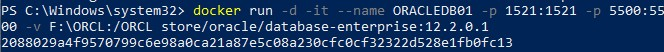
\includegraphics[width=12cm]{./IMAGENES/Docker8_17}
	\end{center}
\end{figure}

\item Para poder realizar consultas de la Base de Datos solo es necesario ejecutar el comando SQL*Plus.
\begin{figure}[htb]
	\begin{center}
		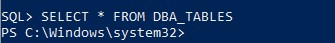
\includegraphics[width=7cm]{./IMAGENES/Docker8_12}
	\end{center}
\end{figure}
\end{enumerate}


\section{CUESTIONARIO}

\begin{enumerate}[a)]
\item ¿Con qué comando(s) puedo iniciar y detener una instancia de Oracle, detalle cada uno de los pasos y opciones, utilizando Docker?\newline


\item ¿Con qué comando(s) puedo iniciar y detener el Listener y el Enterprise manager, detalle cada uno de los pasos y opciones, utilizando Docker?\newline
CREATE DATABASE NAMEDATABASE ON \newline
( FILENAME = N'/var/opt/mssql/data2/NDATABASE.mdf' ),\newline
( FILENAME = N'/var/opt/mssql/data2/NDATABASElog.ldf' )\newline
FOR ATTACH\newline
GO\newline
\item Genere un nuevo contenedor y cree la base de datos con las siguientes características.\newline
Nombre : FINANCIERA \newline
Archivos:
\begin{itemize}
\item DATOS (dbf) : Tamaño Inicial : 50MB, Incremento: 10MB, Ilimitado
\item INDICES (dbf) Tamaño Inicial : 100MB, Incremento: 20MB, Maximo: 1GB
\item HISTORICO (dbf) Tamaño Inicial : 100MB, Incremento: 50MB, Ilimitado
\end{itemize}
\item ¿Cuál sería el script SQL que generaría esta base de datos?
\begin{figure}[htb]
	\begin{center}
		%%\includegraphics[width=10cm]{./IMAGENES/Docker14}
		%%\includegraphics[width=10cm]{./IMAGENES/Docker15}
	\end{center}
\end{figure}
\end{enumerate}

\section{CONCLUSIONES}
Los contenedores nos facilitan una sencilla instalación desde una imagen para poder realizar desplegar la base de ddatos de una aplicación y ademas nos permite poder exportarla para poder ejecutarla en otro equipo sin ninguna complicación.

\section{WEBGRAFIA}
https://es.wikipedia.org/wiki/Docker(software)\newline

\end{document}
